\documentclass{article}
\usepackage{amsmath}
\usepackage{amssymb}
\usepackage{graphicx}
\usepackage{float}
\usepackage{hyperref}
\usepackage{fancyvrb}
\usepackage{enumitem}
\usepackage{matlab-prettifier}
\setlength{\parindent}{0pt}
\graphicspath{{../images/}}

\title{CS663: Digital Image Processing - Homework 4}
\author{Harsh $\vert$ Pranav $\vert$ Swayam}
\date{October 22, 2024} 

\begin{document}

\maketitle
\flushleft
\section*{Homework 4 - Question 3}

\subsection*{(a)}

Let \(\mathbf{A}\) be an \( m \times n \) matrix. The Singular Value Decomposition (SVD) of \(\mathbf{A}\) can be expressed as:

\[
\mathbf{A} = \mathbf{U} \mathbf{S} \mathbf{V}^T
\]

where:

- \(\mathbf{U}\) is an \( m \times m \) orthogonal matrix,

- \(\mathbf{S}\) is an \( m \times n \) diagonal matrix with non-negative entries (singular values),

- \(\mathbf{V}\) is an \( n \times n \) orthogonal matrix.

Considering the product \(\mathbf{A}^T\mathbf{A}\):

\[
\mathbf{A}^T\mathbf{A} = (\mathbf{U} \mathbf{S} \mathbf{V}^T)^T (\mathbf{U} \mathbf{S} \mathbf{V}^T) = \mathbf{V} \mathbf{S}^T \mathbf{U}^T \mathbf{U} \mathbf{S} \mathbf{V}^T = \mathbf{V} \mathbf{S}^T \mathbf{S} \mathbf{V}^T
\]

Since \(\mathbf{V}\) is orthogonal, the eigenvalues of \(\mathbf{A}^T\mathbf{A}\) are the diagonal entries of \(\mathbf{S}^T \mathbf{S}\), which are the squares of the singular values. Thus, the non-zero singular values of \(\mathbf{A}\) are the square roots of the eigenvalues of \(\mathbf{A}^T\mathbf{A}\).

Similarly, for \(\mathbf{A}\mathbf{A}^T\):

\[
\mathbf{A}\mathbf{A}^T = (\mathbf{U} \mathbf{S} \mathbf{V}^T)(\mathbf{U} \mathbf{S} \mathbf{V}^T)^T = \mathbf{U} \mathbf{S} \mathbf{V}^T \mathbf{V} \mathbf{S}^T \mathbf{U}^T = \mathbf{U} \mathbf{S} \mathbf{S}^T \mathbf{U}^T
\]

The eigenvalues of \(\mathbf{A}\mathbf{A}^T\) are also the diagonal entries of \(\mathbf{S} \mathbf{S}^T\), confirming that the non-zero singular values correspond to the square roots of the eigenvalues of both matrices.

\subsection*{(b)}

The Frobenius norm is defined as:

\[
\|\mathbf{A}\|_F = \sqrt{\sum_{i=1}^{m} \sum_{j=1}^{n} |a_{ij}|^2}
\]

Thus, we have:

\[
\|\mathbf{A}\|_F^2 = \sum_{i=1}^{m} \sum_{j=1}^{n} |a_{ij}|^2
\]

From the SVD, we know:

\[
\mathbf{A} = \mathbf{U} \mathbf{S} \mathbf{V}^T
\]

Therefore:

\[
\|\mathbf{A}\|_F^2 = \|\mathbf{U} \mathbf{S} \mathbf{V}^T\|_F^2 = \|\mathbf{S}\|_F^2
\]

Since both \(\mathbf{U}\) and \(\mathbf{V}\) are orthogonal matrices, they do not change the Frobenius norm. The Frobenius norm of a diagonal matrix is simply the sum of squares of its diagonal elements (the singular values):

\[
\|\mathbf{S}\|_F^2 = \sum_{i=1}^{r} \sigma_i^2
\]

Thus, we conclude that:

\[
\|\mathbf{A}\|_F^2 = \sum_{i=1}^{r} \sigma_i^2
\]

\subsection*{(c)}

When attempting to reconstruct \( \mathbf{A} \) from the product \( \mathbf{U} \mathbf{S} \mathbf{V}^T \), the result does not match the original matrix \( \mathbf{A} \), causing confusion. This mismatch arises due to sign inconsistencies in the eigenvectors obtained during the eigen decomposition. 

\subsubsection*{Explanation}

Eigenvectors can have arbitrary signs: if \( \mathbf{u} \) is an eigenvector of \( \mathbf{A} \mathbf{A}^T \) with eigenvalue \( \lambda \), then \( c \mathbf{u} \) is also an eigenvector with the same eigenvalue. This leads to potential sign discrepancies between the left singular vectors in \( \mathbf{U} \) and the right singular vectors in \( \mathbf{V} \), causing \( \mathbf{A} \neq \mathbf{U} \mathbf{S} \mathbf{V}^T \).

\subsubsection*{Mathematical Formulation}
Given a matrix \( \mathbf{A} \in \mathbb{R}^{m \times n} \), we know that the SVD of \( \mathbf{A} \) is given by:
\[
\mathbf{A} = \mathbf{U} \mathbf{S} \mathbf{V}^T
\]

The matrices \( \mathbf{U} \) and \( \mathbf{V} \) are obtained via the eigen decomposition:
\[
\mathbf{A}^T \mathbf{A} = \mathbf{V} \mathbf{S} \mathbf{V}^T \quad \text{and} \quad \mathbf{A} \mathbf{A}^T = \mathbf{U} \mathbf{S} \mathbf{U}^T
\]
where \( \mathbf{S} \) is the diagonal matrix of eigenvalues, and the columns of \( \mathbf{U} \) and \( \mathbf{V} \) are the eigenvectors corresponding to \( \mathbf{A} \mathbf{A}^T \) and \( \mathbf{A}^T \mathbf{A} \), respectively.

\textbf{Sign Inconsistency-}

The issue arises because both \( \mathbf{u} \) and \( -\mathbf{u} \) (similarly, \( \mathbf{v} \) and \( -\mathbf{v} \)) are valid eigenvectors corresponding to the same eigenvalue \( \lambda \). Therefore, the numerical eigen decomposition may return eigenvectors with arbitrary signs. 

When constructing the SVD as \( \mathbf{U} \mathbf{S} \mathbf{V}^T \), any sign discrepancy between corresponding columns of \( \mathbf{U} \) and \( \mathbf{V} \) can result in a mismatch, leading to:
\[
\mathbf{A} \neq \mathbf{U} \mathbf{S} \mathbf{V}^T
\]

\begin{figure}[!htb]
    \centering
    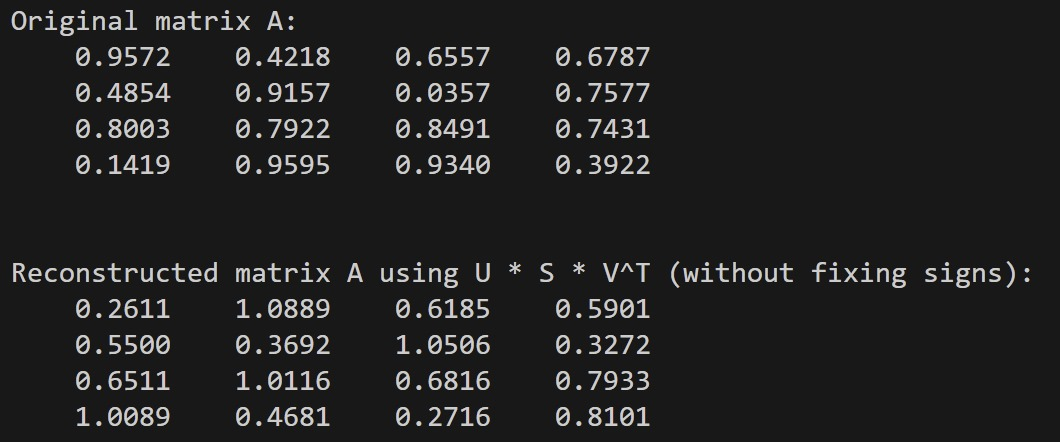
\includegraphics[width=0.75\textwidth]{svd_error.jpg}
    \caption{Incorrect SVD computation}
\end{figure}

\subsubsection*{Resolution of the Sign Inconsistency}
To resolve this, for each \( i \)-th pair of eigenvectors \( \mathbf{u}_i \) (from \( \mathbf{A} \mathbf{A}^T \)) and \( \mathbf{v}_i \) (from \( \mathbf{A}^T \mathbf{A} \)), adjust the signs as follows:
\[
\text{If } \operatorname{sign}(\mathbf{u}_i^T \mathbf{A} \mathbf{v}_i) < 0, \text{ set } \mathbf{u}_i \leftarrow -\mathbf{u}_i
\]
This ensures the correct reconstruction \( \mathbf{A} = \mathbf{U} \mathbf{S} \mathbf{V}^T \).

\begin{figure}[!htb]
    \centering
    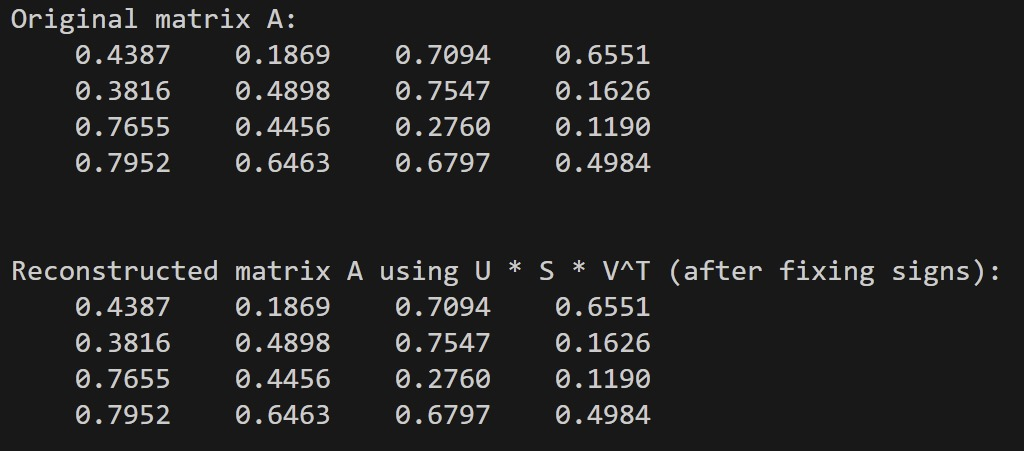
\includegraphics[width=0.75\textwidth]{svd_corrected.jpg}
    \caption{Corrected SVD computation}
\end{figure}

\subsection*{(d)}

\subsubsection*{(i)}

Considering there are appropriate number of elements in the vector,

$$\mathbf{y}^T\mathbf{P}\mathbf{y} = \mathbf{y}^T\mathbf{A}^T\mathbf{A}\mathbf{y} = (\mathbf{A}\mathbf{y})^T(\mathbf{A}\mathbf{y}) = \|\mathbf{A}\mathbf{y}\|^2 \geq 0$$
$$\implies \mathbf{y}^T\mathbf{P}\mathbf{y} \geq 0$$

Similarly, for the matrix \( \mathbf{Q} \), we have:

$$\mathbf{z}^T\mathbf{Q}\mathbf{z} = \mathbf{z}^T\mathbf{A}\mathbf{A}^T\mathbf{z} = (\mathbf{A}^T\mathbf{z})^T(\mathbf{A}^T\mathbf{z}) = \|\mathbf{A}^T\mathbf{z}\|^2 \geq 0$$
$$\implies \mathbf{z}^T\mathbf{Q}\mathbf{z} \geq 0$$

Now, the eigenvalues of a positive semi-definite matrix are non-negative. 
And, since \( \mathbf{P} \) and \( \mathbf{Q} \) are positive semi-definite matrices, as shown above, the eigenvalues of \( \mathbf{P} \) and \( \mathbf{Q} \) are non-negative.

\textbf{Proof:} Let \( \lambda \) be an eigenvalue of \( \mathbf{P} \) and \( \mathbf{v} \) be the corresponding eigenvector. Then:

$$\mathbf{P}\mathbf{v} = \lambda \mathbf{v}$$
$$\implies \mathbf{v}^T\mathbf{P}\mathbf{v} = \lambda \mathbf{v}^T\mathbf{v}$$
$$\implies \mathbf{v}^T\mathbf{P}\mathbf{v} = \lambda$$

Since \( \mathbf{P} \) is positive semi-definite, \( \mathbf{v}^T\mathbf{P}\mathbf{v} \geq 0 \), which implies \( \lambda \geq 0 \). Thus, the eigenvalues of \( \mathbf{P} \) are non-negative.

Similarly, for \( \mathbf{Q} \), let \( \mu \) be an eigenvalue of \( \mathbf{Q} \) and \( \mathbf{w} \) be the corresponding eigenvector. Then:

$$\mathbf{Q}\mathbf{w} = \mu \mathbf{w}$$
$$\implies \mathbf{w}^T\mathbf{Q}\mathbf{w} = \mu \mathbf{w}^T\mathbf{w}$$
$$\implies \mathbf{w}^T\mathbf{Q}\mathbf{w} = \mu$$

Since \( \mathbf{Q} \) is positive semi-definite, \( \mathbf{w}^T\mathbf{Q}\mathbf{w} \geq 0 \), which implies \( \mu \geq 0 \). Thus, the eigenvalues of \( \mathbf{Q} \) are non-negative.

\subsubsection*{(ii)}

Let \( \mathbf{u} \) be an eigenvector of \( \mathbf{P} \) with eigenvalue \( \lambda \). Then:

$$\mathbf{P}\mathbf{u} = \lambda \mathbf{u}$$
$$\therefore \mathbf{A}\mathbf{P}\mathbf{u} = \mathbf{A}(\lambda \mathbf{u}) = \lambda \mathbf{A}\mathbf{u}$$
$$\implies \lambda \mathbf{A}\mathbf{u} = \mathbf{A}\mathbf{A}^T\mathbf{A}\mathbf{u} = (\mathbf{A}\mathbf{A}^T)\mathbf{A}\mathbf{u} = \mathbf{Q}\mathbf{A}\mathbf{u} $$

Thus, \( \mathbf{A}\mathbf{u} \) is an eigenvector of \( \mathbf{Q} \) with eigenvalue \( \lambda \).

Similarly, let \( \mathbf{v} \) be an eigenvector of \( \mathbf{Q} \) with eigenvalue \( \mu \). Then:

$$\mathbf{Q}\mathbf{v} = \mu \mathbf{v}$$
$$\therefore \mathbf{A}^T\mathbf{Q}\mathbf{v} = \mathbf{A}^T(\mu \mathbf{v}) = \mu \mathbf{A}^T\mathbf{v}$$
$$\implies \mu \mathbf{A}^T\mathbf{v} = \mathbf{A}^T\mathbf{A}\mathbf{A}^T\mathbf{v} = (\mathbf{A}^T\mathbf{A})\mathbf{A}^T\mathbf{v} = \mathbf{P}\mathbf{A}^T\mathbf{v} $$

Thus, \( \mathbf{A}^T\mathbf{v} \) is an eigenvector of \( \mathbf{P} \) with eigenvalue \( \mu \).

The number of elements in \( \mathbf{u} \) and \( \mathbf{v} \) are the same as the number of rows in \( \mathbf{P} \) and \( \mathbf{Q} \), respectively.

\subsubsection*{(iii)}

$$\mathbf{Q}\mathbf{v}_i = \mu_i \mathbf{v}_i$$
$$\implies \mathbf{A}\mathbf{A}^T\mathbf{v}_i = \mathbf{A}(\mathbf{A}^T\mathbf{v}_i) = \mu_i \mathbf{v}_i$$
$$\implies \mathbf{A}\mathbf{u}_i = \frac{\mu_i \mathbf{v}_i}{\|\mathbf{A}^T\mathbf{v}_i\|}$$

Let \( \gamma_i = \frac{\mu_i}{\|\mathbf{A}^T\mathbf{v}_i\|} \). Then:

$$\mathbf{A} \mathbf{u}_i = \gamma_i \mathbf{v}_i$$
where, \( \gamma_i \) is non-negative because \( \mu_i \) is real, non-negative and \( \|\mathbf{A}^T\mathbf{v}_i\| \) is non-negative.

Thus, there exists a real, non-negative \( \gamma_i \) such that \( \mathbf{A} \mathbf{u}_i = \gamma_i \mathbf{v}_i \).

\subsection*{(iv)}

$$\mathbf{A}\mathbf{u}_i = \gamma_i \mathbf{v}_i \quad \forall 1 \leq i \leq m$$
$$\mathbf{A}\mathbf{u}_i = 0 \quad \forall m+1 \leq i \leq n$$
$$\implies \mathbf{A} \mathbf{V} = \mathbf{U} \mathbf{\Gamma}$$
where, \( \mathbf{V} \) is an \( n \times n \) orthonormal matrix with columns as \( \mathbf{v}_i \), \( \mathbf{U} \) is an \( m \times m \) matrix with columns as \( \mathbf{u}_i \), and \( \mathbf{\Gamma} \) is an \( m \times n \) matrix with diagonal entries as \( \gamma_i \) and all other entries as 0.

$$\implies \mathbf{A} = \mathbf{U} \mathbf{\Gamma} \mathbf{V}^T$$
where the values in \( \mathbf{\Gamma} \) are non-negative as proved above.

\end{document}